\chapter{Literature Review}\label{Literature Review}

\section{The Media}

\subsection{Role of the Media in a crisis}\label{Role of the Media in a crisis}

TODO

\subsection{French Press}\label{chap:French Press}

TODO: possibly include some history of french press, AFP and more
% Find what the role of the press is, should be specifically in the context of important, hurtful events
%How the people see the covid 19 pandemic

\section{Sentiment Analysis}\label{Sentiment Analysis}

Sentiment Analysis (or opinion mining), is "the task of finding the opinions of authors about specific entities" \citep{feldman2013techniques}. It is a sub-field of Natural Language Processing (NLP) which has been growing in interest on a worldwide scale for over 15 years thanks to its vast range of use cases (Figure \ref{fig:sentiment interest}).

\begin{figure}[h!]
      \centering
      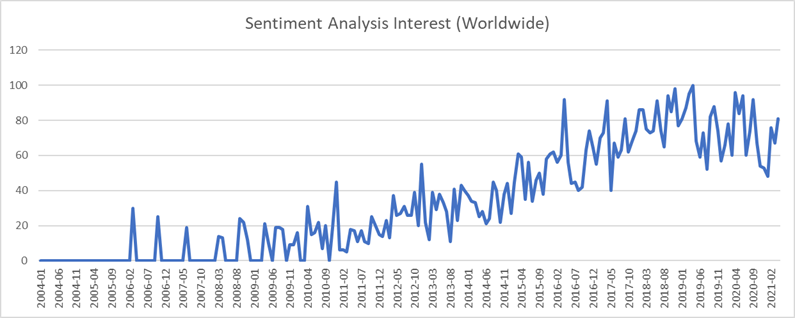
\includegraphics[scale=0.65]{lit_review/sentiment_analysis_interest.png}
      \caption{Sentiment Analysis Interest}
      \label{fig:sentiment interest}
      \emph{Source: Google Trends}
\end{figure}

In fact, sentiment analysis has been used in a wide range of topics, including political analyses of social and news media \citep{ahmad2011new}, stock market behaviors \citep{rao2012analyzing,li2014news}, customer sentiment \citep{cambria2013new,mouthami2013sentiment}, fake news detection \citep{bhutani2019fake} and countless more applications.

Languages are full of ambiguity and in particular the french language as some words can have drastically different meanings even though they are written the same, or adding an accent from a large variety of options can drastically change a words meaning. On top of this, it was found that a select set of words make up the majority of text, in fact, using a frequency-rank, it was found that the first 100 words make up for about 50\% of all of the words in a text cluster \citep{ahmad2007being}, this observation means that the interpretation of these highly frequent words is key to extracting sentiment proxies from text. While short text such as tweets \citep{chandrasekaran2020topics} or customer reviews can include a single sentiment or topic. It is not always the case and as the length of text grows more and more conflicting opinions are likely found. A simple example of this can be found on a customer review for a product: "I liked using the product, however I wish it didn't break after a day" where clearly both a positive and negative sentiment can be extracted from this review. This shows that there are multiple ways to perform sentiment analysis on text. Document-level computes the overall sentiment of a piece of text such as a tweet or a review, on the other hand, a sentence-level analysis approach can also be taken where a distinction is made between factual sentences (objective phrases) and subjective sentences which mostly contain opinions (subjective phrases) \citep{wilson2009recognizing}. A sentence-level approach is often used for tasks such as text summarizing, on the other hand, a document-level approach is often used for reviews or social media posts. 

Thankfully, some NLP techniques have now been standardised to help with these issues. One of the most important ones being the use of stemming or lemmatising. Both of these techniques transform words into a more basic version of that word, 

TODO: detail sections on lexicon / ml, lemmatization vs stemming and more (note: may be worth mentioning regexp)

\subsection{TODO}

TODO: lemmatization stemming, ml / lexicons. SpaCy \& treetagger lemmatizer. Etc
%\subsection{Lemmatization}
\label{lemmatization}

%compare treetagger and SpaCy -- show mean scores.
% look into ML vs Lexicon, stemming vs lemmas
% look into language issue English vs others
% french dictionaries

\section{French Lexica}\label{French Lexicons}

\subsection{FEEL}\label{chap: feel}

TODO

\subsection{Diko}\label{chap: diko}

TODO

\subsection{Polarimots}\label{chap: polarimots}

TODO

\section{Statistical Methods}\label{Statistical Methods}

The use of various statistical methods represent a key element for this thesis, as specified in the research objectives (Chapter \ref{chap: Research Objectives}). Such methods provide the link between observed values and identifying potential relationships. The various statistical methods used throughout this thesis will be introduced in the following sections.

\subsection{Core Statistics}

This first section introduces key, core statistic measures which are used throughout this thesis.

\subsubsection{Mean}

The mean is a very well known statistical measure which consists of the sum of the deviation of all of the values in a sample by the size of that sample. In other words, it is the average value in a sample. It is commonly referred to as $\bar{x}$ for a sample as well as $\mu$ for a population. It can be written as such:

\begin{equation}
    \mu = \bar{x} = \frac{1}{N}\sum^{N}_{i=1} x_{i}
\end{equation}
Where N is the sample size and $x_{i}$ represents the ith value in the sample.

\subsubsection{Variance and Standard Deviation}

The standard deviation and variance are related. A common symbol for the standard deviation is $\sigma$ for a population and $S$ for a sample. Given the standard deviation $S$ or $\sigma$ then the variance is its squared value: $S^{2}$ or $\sigma^{2}$.

The standard deviation measures how much data diverges from the mean. A low value indicates that the data is clustered around the mean, on the other hand a high standard deviation indicates that the sample is more spread out. The variance also measures how distributed data is relative to the mean in the same manner, except in much larger values as it is squared.

The mathematical formulas for computing the standard deviation and variance for a sample are the following:
\begin{equation}
    S = \sqrt{\frac{\sum_{i=1}^{N}(x_{i} - \bar{x})^{2}}{N - 1}}
\end{equation}
\begin{equation}
    S^2 = \frac{\sum_{i=1}^{N}(x_{i} - \bar{x})^{2}}{N - 1}
\end{equation}

\subsubsection{Skewness}

Similar to the variance and standard deviation, the skewness also measures data distribution. The skewness measures the degree of asymmetry from a normal distribution, in other words, it quantifies the difference between a sample distribution and the normal distribution.

Hence, the skewness for a normal distribution is 0. A positive skewness indicates that the data is skewed to the right, in other words the right tail is longer than the left. On the other hand, a negative skewness indicates that the data is skewed to the left. Figure \ref{skewness fig} illustrates this concept. Mathematically, it is written as such:

\begin{equation}
    skewness = \frac{\sum_{i=1}^{N}(x_{i} - \bar{x})^{3}}{(N - 1) * S^{3}}
\end{equation}
Where N is the sample size, $x_{i}$ is the ith data point from the sample, $\bar{x}$ is the mean and $S$ is the standard deviation.

\begin{figure}[h!]
      \centering
      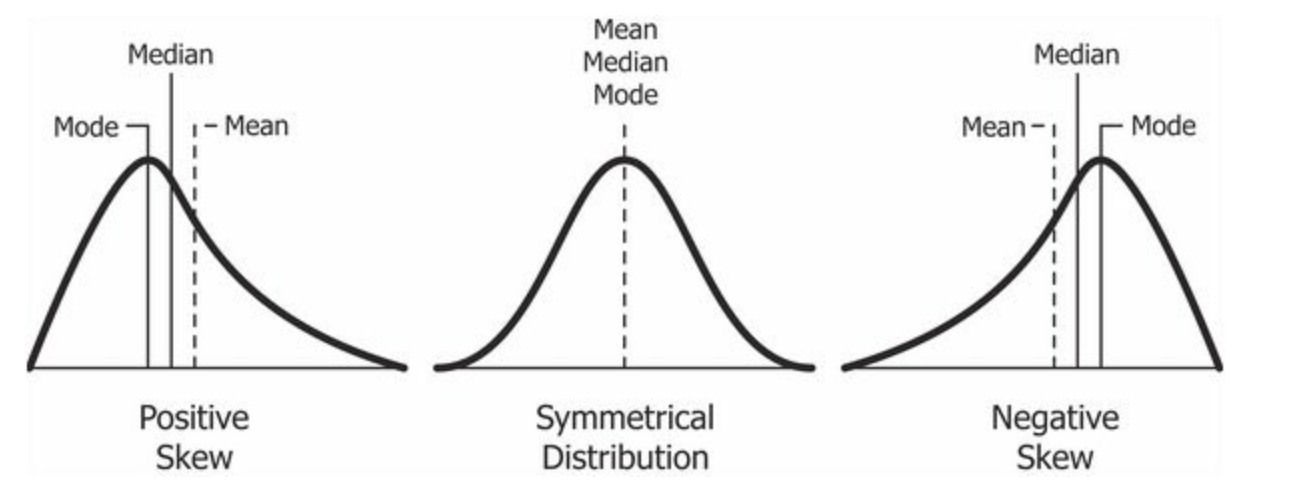
\includegraphics[scale=0.8]{lit_review/skewness.png}
      \caption{Skewness Visualisation}
      \label{skewness fig}
      \emph{Source: Wikipedia}
\end{figure}

\subsubsection{Kurtosis}

Kurtosis is a measure of whether a sample is heavily tailed or lightly tailed relative to a normal distribution. A high kurtosis value infers that a data set will have a large amount of outliers. On the other hand a low kurtosis value indicates a data set with very few outliers. The kurtosis for a standard normal distribution is 3, hence a metric often used is referred to as the "excess kurtosis" and takes the value $kurtosis - 1$.

Mathematically, the kurtosis value is calculated as such:
\begin{equation}
    kurtosis = \frac{1}{N - 1} \frac{\sum_{i=1}^{N}(x_{i} - \bar{x})^{4}}{S^{4}}
\end{equation}

\subsubsection{P-Value}

The P-Value is used in null hypothesis significance testing. Assuming a null hypothesis $H_{0}$, a hypothesis of no difference, and a second hypothesis $H_{1}$, representing the opposite of the null hypothesis. The P-Value is the probability of finding greater results when the null hypothesis $H_{0}$ is true. A level of significance is picked, typically one of 0.1, 0.05 or 0.01. A p-value below the threshold, then we can conclude that there is significant evidence to reject the null hypothesis $H_{0}$. This study uses a significance level of 5\% (p-value of 0.05) by default unless specified otherwise.

\subsubsection{Correlation}

This study makes use of the Pearson product-moment correlation coefficient. Correlation (r) quantifies linear relationship between two data sets. Its values ranges between -1 and 1. A correlation value of zero indicates no linear relationship between the two sets of data. A positive correlation indicates that both variables move in the same direction, it shows that when one becomes larger or smaller, so does the other. On the other hand, a negative correlation shows the opposite: both variables move in the opposite directions. 
A larger distance between zero and the correlation value indicates a stronger relationship, this is true for both positive and negative correlations. The coefficient can be computed using the formula below.

\begin{equation}
    r = \frac{\sum_{i=1}^{N}(x_{i} - \bar{x})(y_{i} - \bar{y})}{\sqrt{\sum_{i=1}^{N}(x_{i} - \bar{x})^{2}\sum_{i=1}^{N}(y_{i} - \bar{y})^{2}}}
\end{equation}
Note that both sets of data must be of the same size. Here N is the sample size of both x and y data sets, $x_{i}$ and $y_{i}$ are the ith data point for data sets x and y respectively, finally $\bar{x}$ and $\bar{y}$ are the means for both data sets.

\subsubsection{Z-Score}

The Z-Score (Z), also known as the standard score, is a value which shows a measure of the a value's relationship to the mean of the data set it belongs to. It represents the number of standard deviations by which a value is above or below the mean value.

\begin{equation}
    Z = \frac{x - \bar{x}}{S}
\end{equation}
Where x is a value of the data set, $\bar{x}$ is the mean and $S$ is the standard deviation.

\subsection{TODO: VAR / Causality Test}
TODO
%- main statistical measures
%- correlation 
%- statistical significance (look into durbin watson), hypothesis testing
%- F-statistic with p-value
%- unit root test
%- R\^2
%- granger causuality test
%- VAR ?
%- variance, z-score
